\documentclass[10pt,twocolumn,letterpaper]{article}

\usepackage{cvpr}
\usepackage{times}
\usepackage{epsfig}
\usepackage{graphicx}
\usepackage{amsmath}
\usepackage{amssymb}

% Include other packages here, before hyperref.

% If you comment hyperref and then uncomment it, you should delete
% egpaper.aux before re-running latex.  (Or just hit 'q' on the first latex
% run, let it finish, and you should be clear).
\usepackage[breaklinks=true,bookmarks=false]{hyperref}

\cvprfinalcopy % *** Uncomment this line for the final submission

\def\cvprPaperID{****} % *** Enter the CVPR Paper ID here
\def\httilde{\mbox{\tt\raisebox{-.5ex}{\symbol{126}}}}

% Pages are numbered in submission mode, and unnumbered in camera-ready
%\ifcvprfinal\pagestyle{empty}\fi
\setcounter{page}{1}
\begin{document}

%%%%%%%%% TITLE
\title{Multi-Task Neural Network for Brain Tumor Segmentation and Survival Rate Prediction on BraTS Dataset}
\author{Cecchin Andrea\\
{\tt\scriptsize andrea.cecchin.5@studenti.unipd.it}\\
% For a paper whose authors are all at the same institution,
% omit the following lines up until the closing ``}''.
% Additional authors and addresses can be added with ``\and'',
% just like the second author.
% To save space, use either the email address or home page, not both
\and
Dugo Alberto\\
{\tt\scriptsize alberto.dugo@studenti.unipd.it}\\
\and
Soldà Matteo\\
{\tt\scriptsize matteo.solda.1@studenti.unipd.it}\\
}
\maketitle
%\thispagestyle{empty}

%%%%%%%%% ABSTRACT
\begin{abstract}
    This paper presents a unified deep learning framework based on the U-Net architecture for the simultaneous tasks of brain tumor segmentation and survival prognosis. Utilizing the publicly available BraTS Challenge dataset for training and evaluation, the proposed model leverages multimodal MRI data to generate precise segmentations of tumor regions and to predict patient survival duration. By addressing these two critical challenges in clinical oncology within a single architecture, the approach demonstrates the potential of integrated deep learning solutions for comprehensive and clinically relevant analysis of brain tumors.
\end{abstract}

%%%%%%%%% BODY TEXT
\section{Introduction}
CBTRUS\cite{CBTRUSTumors2022} maintains and regularly updates a registry of malignant and non-malignant brain tumors.
In global data, the incidence of malignant brain tumors is approximately 3.5 per 100,000 people. This incidence increases to 3.9 for the male population and 3.1 for the female population. This indicates that approximately 173,699 men and 148,032 women are diagnosed with brain tumors each year, for a total of 321,731 individuals. The average annual mortality in the United States alone between 2017 and 2021 was 4.41 per 100,000 people. This represents a death of 17,411 people per year, or 48 deaths per day.


Brain Tumor Segmentation Challenge is an annual competition, firstly launched by the Perelman School of Medicine\cite{BraTSChallenge} in 2012, focused on evaluating the performance of algorithms in tasks related to the segmentation of brain tumors in multimodal MRI scans. In particular, our work focused on the following tasks proposed by the competition:

\begin{itemize}
	\item Segmentation of Gliomas: it is the task of recognizing a tumor region, if present. It requires the segmentation of the three typical regions which characterize a brain tumor:
    \begin{itemize}
        \item Enhancing Tumor: it is the region of a brain tumor characterized by the presence of a disrupted blood-brain barrier.
        \item Peritumoral Edema: it is the swelling of tissue surrounding a brain tumor, caused by the accumulation of fluid.
        \item Necrotic and Non-Enhancing Tumor Core: it is the central region of a brain tumor that contains dead tissue.
    \end{itemize}	
	\item Prediction of Overall Survival: this task involves predicting the survival rate of patients based on their MRI scans.
\end{itemize}

Being able to correctly identify and classify tumor areas is a highly important task, because it increase the survival rate of patients. Despite that, those tasks are extremely challenging. The difficulty of these tasks, and the reason why tumor segmentations are performed by human experts, lies in the challenge of visualizing certain tumor areas in MRI scans.

Indeed, while peritumoral edema is easily visible even without image preprocessing or contrast modification, the Enhancing Tumor is only visible in post-contrast scans, where it appears brighter. Even more difficult is the segmentation of the Necrotic and Non-Enhancing Tumor Core, which does not show contrast enhancement in MRI scans.

Modeling and training a deep neural network to perform these tasks would decrease the time required to accurately identify tumor regions in MRI scans, potentially increasing the accuracy of human-made segmentations. Additionally, predicting survival rates could be useful in defining an irreversible clinical condition, where tumor segmentations and surgery attempts would be futile.

%------------------------------------------------------------------------
\section{Related Works}

The most cited work about tumor segmentation made through Deep Learning Networks is the one wirtten by Havaei et Al.\cite{HAVAEI201718} that presents a Convolutional Neural Network that exploits local features and some global contextual features at the same time. This specific model is implemented through a fully connected layer which allows a 40 fold speed up and a 2-phase training procedure. The overall dice score of this model is of 0.86 (complete regions), 0.86 (core regions) and 0.77 (enhancing tumor regions).
There is also an article made by Gordillo et Al.\cite{GORDILLO20131426} that explore the state of the art of MRI brain tumor segmentation, comparing various models.

%-------------------------------------------------------------------------

\section{Dataset}

For this project, we used the official dataset\cite{BraTSdataset} provided for the BraTS Challenge held in 2020, obtained from the Kaggle dataset repository. The data it contains, consisting of the combination of 19 different smaller datasets created using various clinical protocols and scanners, include MRI scans from 494 patients.

For each patient, four different three-dimensional brain scans are provided. T1-weighted MRI is a type of scan that emphasizes the anatomical details of the brain. It provides good contrast between gray matter and white matter, making brain structures clearly visible. T1 contrast-enhancing, on the other hand, is a T1 image acquired after the administration of a gadolinium-based contrast agent. The contrast accumulates in areas with high vascular permeability, such as tumors, which absorb the contrast and appear brighter than the surrounding tissues. The T2 scan highlights water-rich areas, such as edema, while T2-FLAIR, or simply FLAIR (Fluid Attenuated Inversion Recovery), is a variant of T2 in which the cerebrospinal fluid signal is suppressed, allowing better visualization of brain lesions.

\begin{figure}[H]
    \centering
    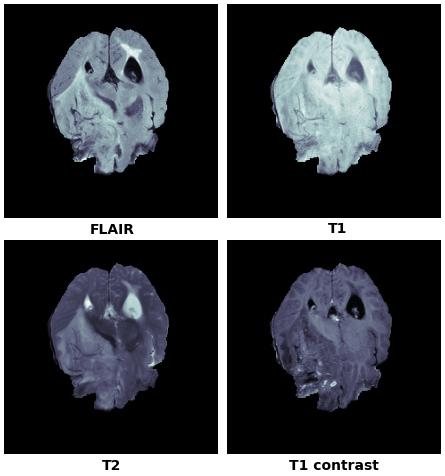
\includegraphics[width=0.6\linewidth]{img/example_MRI.png}
    \caption{Example of an MRI scan with FLAIR, T1, T2 and T1 contrast-enhancing.}
\end{figure}

The images provided in the dataset have been preprocessed to facilitate their use. Specifically, all scans have been realigned and resampled to the same voxel size of 1 mm³. Additionally, all non-brain tissues, such as the skull and scalp, have been removed.

For all patients in the training set, totaling 369, manual segmentations of tumor areas were created, verified, and validated by expert neuroradiologists. These segmentations were used during the training and validation phases of the model as the "ground truth" for the segmentations produced by our neural network.

\begin{figure}[H]
    \centering
    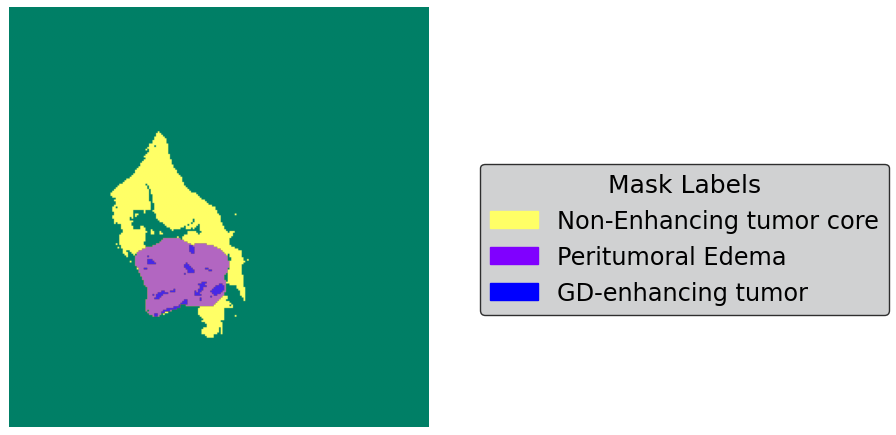
\includegraphics[width=0.8\linewidth]{img/groundtruth_example.png}
    \caption{A colored version of the manual segmentation provided for a patient in the training set.}
\end{figure}

To complete the dataset, a list of all patients who did not survive the tumor was provided, including their age at the time of death and the number of days from the MRI scans to that day.

%-------------------------------------------------------------------------

\section{Method}
Our model implements a customized 3D U-Net architecture specifically designed for volumetric brain tumor segmentation in multimodal MRI scans.

\subsection{Architecture}
We developed an improved 3D U-Net variant with an exceptionally lightweight structure, optimized for efficient tumor subregion delineation. The network is designed to be as compact as possible while preserving high segmentation accuracy. It comprises a total of 340,596 parameters, corresponding to approximately 1.30 MB of memory during inference (assuming 32-bit floating-point precision).
The architecture features three resolution levels in the encoder path and a corresponding symmetric decoder path, connected via skip connections to preserve spatial information. The encoder is composed of sequential blocks that capture hierarchical features through $3\times3\times3$ convolutions, followed by Instance Normalization and LeakyReLU activations. Downsampling between resolution levels is implemented using 3D max pooling with a stride of 2.
Each encoder block adopts a residual-like structure, with dual convolutional layers that facilitate improved gradient flow during training. The decoder path restores spatial resolution using 3D transposed convolutions (kernel size 2, stride 2) for upsampling. Features from the encoder are concatenated with the upsampled representations via skip connections, effectively combining low-level spatial details with high-level semantic features. Dynamic padding is applied to ensure precise spatial alignment during concatenation.
To mitigate overfitting, a dropout layer with a rate of $0.3$ is inserted prior to the final $1\times1\times1$ convolutional layer, which maps feature representations to the output segmentation classes. Model weights are initialized using Kaiming initialization, which is well-suited for networks employing LeakyReLU activations.
The network produces probability maps for four target classes (background and three tumor subregions), while preserving the original spatial dimensions of the input volume. This architecture achieves a strong balance between computational efficiency and segmentation performance, making it well-suited for clinical deployment, especially in resource-constrained environments.

\subsection{Input Preparation}
Our model processes the full 3D volumetric MRI scans from the BraTS 2020 dataset. Each input sample consists of four co-registered modalities (T1, T1ce, T2, and FLAIR) with dimensions $4 \times 240 \times 240 \times 155$, where the first dimension represents the input channels. Prior to feeding the data into our network, we applied intensity normalization independently for each modality using z-score standardization, ensuring each modality had zero mean and unit variance within the brain region.

To address memory constraints while preserving the volumetric context essential for accurate segmentation, 
we implemented patch-based processing during both training and inference. 
%--------TO UNDERSTAND IF IT IS IN THIS WAY--------
%We extracted overlapping sub-volumes of size $4 \times 128 \times 128 \times 64$ with a stride of 32 voxels along each spatial dimension. This approach allows our network to capture sufficient 3D contextual information while maintaining computational feasibility.
%For dataset partitioning, we employed a patient-level stratified split, allocating 80\% of cases to the training set and 20\% to the validation set while ensuring balanced distribution of tumor types and volumes across partitions.

\subsection{Loss Function}


\section{Experiments}

All text must be in a two-column format. 

%-------------------------------------------------------------------------
\section{Conclusions}

All text must be in a two-column format. 

%-------------------------------------------------------------------------

{\small
\bibliographystyle{ieee_fullname}
\bibliography{bibliography}
}

\end{document}
